\documentclass{beamer}
% personal data
\date{\today}


% language
\usepackage{polyglossia}
\setmainlanguage{english}
\setotherlanguages{german}
\usepackage{microtype}
\usepackage{dcolumn}

\usepackage[style=numeric,
			natbib=true,
			backend=biber]{biblatex}		%Bibliographie
\usepackage[autostyle=true,
			 german=quotes]
			 {csquotes}					%Anführungszeichen
\usepackage{blindtext}


%math and theorems
\usepackage{amsmath}
\usepackage{amssymb}
\usepackage{amsopn}					%Matheoperatoren
\usepackage[amsmath,thmmarks,hyperref]{ntheorem}
\usepackage{mathtools}
\usepackage{mathdots}					%Punkte
\usepackage{dsfont}
\usepackage{upgreek}					%Griechische Buchstaben
\usepackage{bbm}						%Mengensymbol
\usepackage{physics}					%Physiksymbole
\usepackage{relsize}						%Größenangaben
\usepackage[separate-uncertainty,
			per-mode=symbol]
			{siunitx}					%Einheiten
%\usepackage{tikz}						%Zeichnen
\usepackage{upgreek}					%Griechische Buchstaben
\usepackage{enumitem}
\setlist{nolistsep}


%useful packages
%\usepackage{geometry}
\usepackage{xcolor}
\usepackage{graphicx}
\usepackage{float}
\usepackage{csquotes}
\usepackage{todonotes}
\usepackage{booktabs}
\usepackage{array}
\usepackage[labelfont=bf]{caption}
\usepackage{wrapfig}
\usepackage{enumitem}
%\usepackage{xr} % cross referencing
%\usepackage{titling}
%\usepackage{titlesec}
%\usepackage[Bjornstrup]
%			{fncychap}					%Kapitellayout


\setmainfont{Linux Libertine O}
\setsansfont{Linux Biolinum O}

\usepackage{scrhack}					%Verbesserung Pakete
\usepackage{xltxtra}						%fontec


\newcommand{\im}{\mathrm{i}}
\newcommand{\e}{\mathrm{e}}
\renewcommand{\pi}{\uppi}
\renewcommand{\epsilon}{\varepsilon}


\addbibresource{bibliography.bib}

%color settings
\definecolor{myred}{RGB}{196,19,47} 
\definecolor{myblue}{RGB}{0,139,139}


%appendix
\usepackage[toc,page]{appendix}

%killing indent
\setlength{\parindent}{0pt}
\usepackage{multicol}
\usepackage{siunitx}
\usepackage{hyperref}


\title{Atmosphärische Spurensuche}
\author{Aaron Mielke \& Thomas Ackermann}
\date{\today}


\begin{document}

\maketitle

% \tableofcontents

\begin{frame}
\frametitle{Einführung}
    \section{Theoretische Grundlagen}
Aufbau der Atmosphäre \\
    Beschränkung auf die Spurengase \ch{O3}, \ch{O4} und \ch{NO2} 
\end{frame}


\begin{frame}
\frametitle{Messgrößen}
    \begin{itemize}
        \item Konzentration: Moleküle pro Volumeneinheit
        \item Mischverhältnis: Relativer Anteil von Spurengas zu Luftmenge
        \item Columnd density: $CD = \int \rho (s) \dd s$
    \end{itemize}
\end{frame}


\begin{frame}
    \frametitle{Inhaltsangabe}
    Theoretische Grundlagen\\
    \vfill
    Labormessungen\\
    \vfill
    Atmosphärische Messungen 
\end{frame}


\begin{frame}
    \frametitle{DOAS}
    \section{Theoretische Grundlagen}
    \begin{columns}
    \column{.6\textwidth}
    \begin{itemize}
        \item[-] Verwendung: Konzentration von Spurengasen bestimmen
        \item[-] Benutze Chrakteristische Profile von Molekülen
    \end{itemize}
    %\hfill
    \column{0.4\textwidth}
    \begin{minipage}{80mm}
        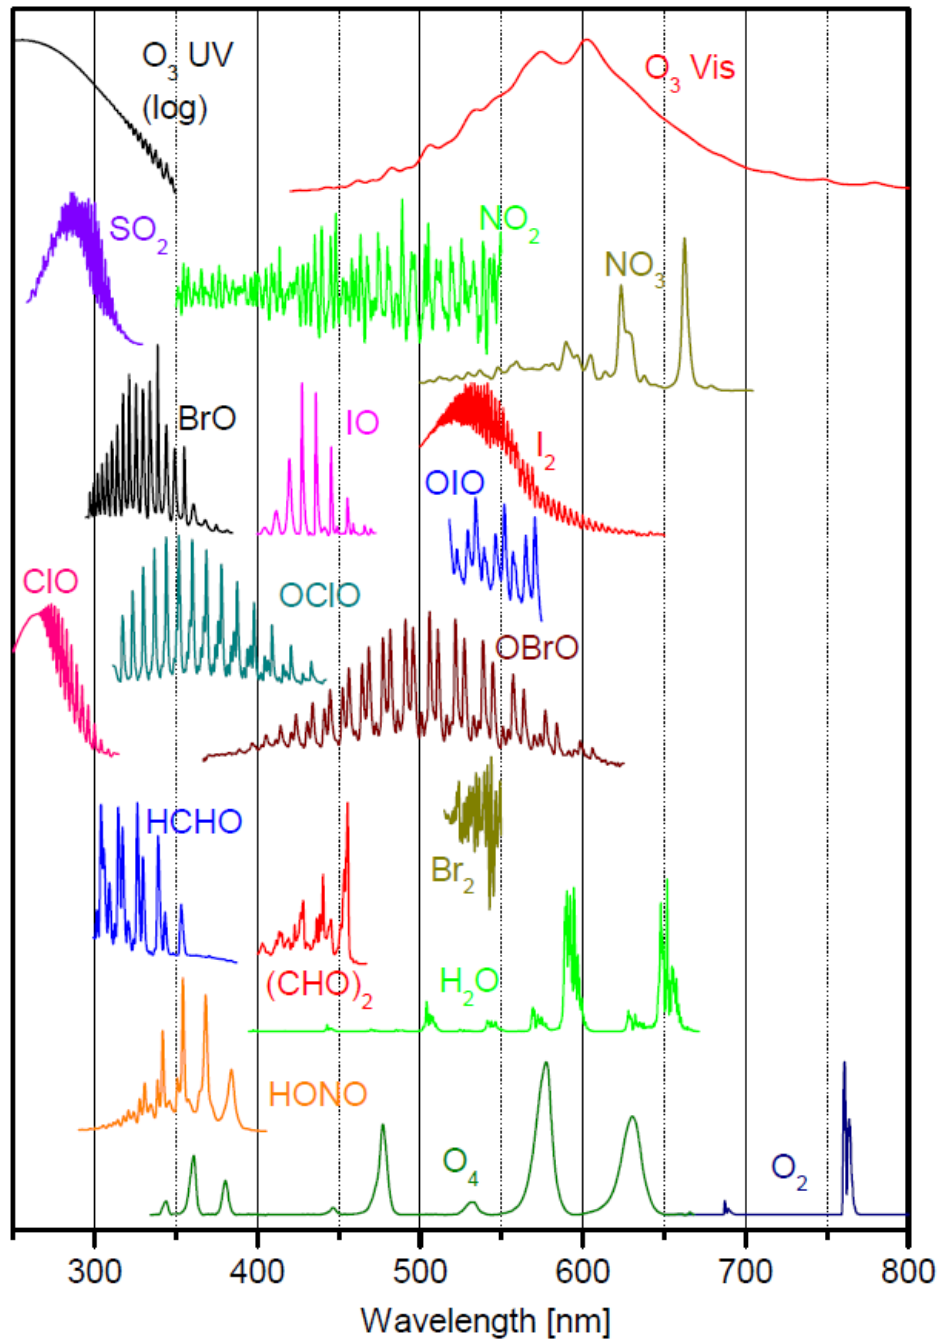
\includegraphics[width=0.5\textwidth]{fig/gas_spectra.png}
    \end{minipage}
    \end{columns}
\end{frame}

\begin{frame}
    \frametitle{Lambert-Beer}
    \begin{figure}[h]
        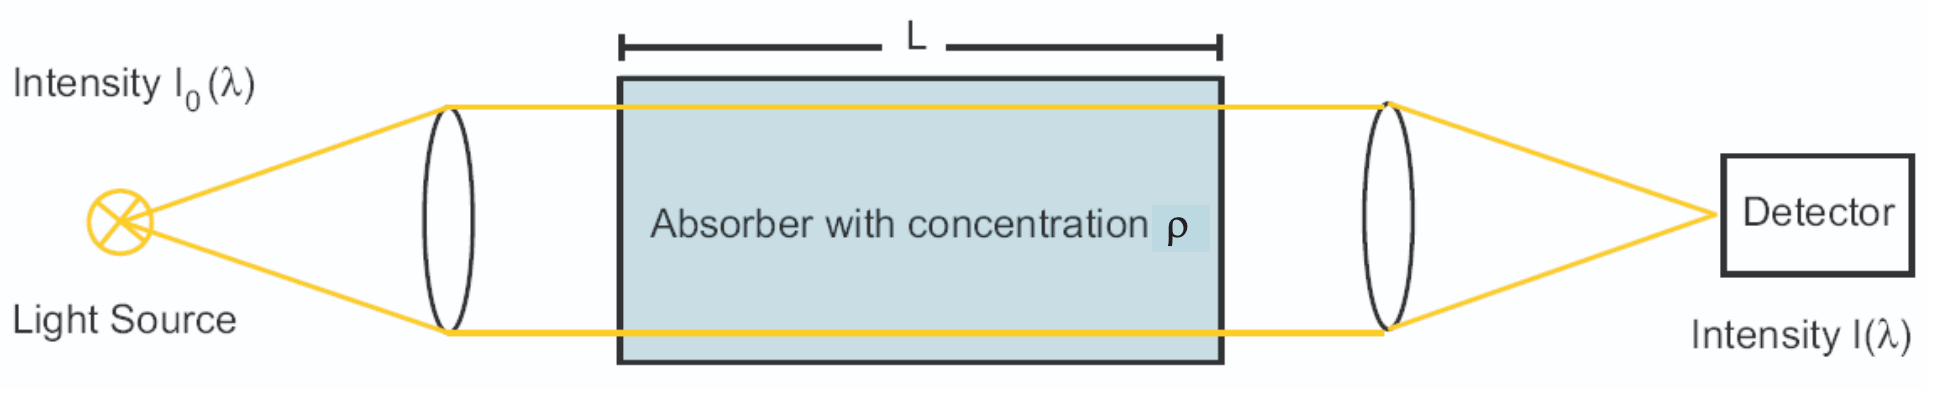
\includegraphics[width=0.5\textwidth]{fig/lambert_beer.png}
    \end{figure}
\pause
    \begin{align}
    I(\lambda, L) = I_0 (\lambda) \exp (- \rho  L \sigma (\lambda) )
    \end{align}
    \begin{itemize}
        \item $L$ Länge des Mediums
        \item $\rho$ Dichte
        \item $\sigma (\lambda)$ Absorptionswirkungsquerschnitt
    \end{itemize}
\end{frame}


\begin{frame}
    \frametitle{DOAS-Fit}
    Forme Lambert-Beer um:
\begin{align}
    \tau = \log \frac{I}{I_0} = - \rho L \sigma (\lambda).
\end{align}
$\tau$ : Optische Dichte\\
Erstelle Fit durch minimierung von
    \begin{align}
        \chi^2 = ( \log \frac{I_0}{I} - \rho L \sigma )^2. 
    \end{align}
\end{frame}


\begin{frame}
    \frametitle{Kurzband Effekte}
Fraunhofer Referenzspektrum
    \begin{itemize}
        \item Berücksichtigung der Strukturen der Sonne
    \end{itemize}
    Ring-Effekt
    \begin{itemize}
        \item Inelastische Raman-Streuung
        \item Wellenlängen ändern siich
    \end{itemize}
\end{frame}

\begin{frame}
    \frametitle{Breitband Effekte}
    \begin{itemize}
        \item Streuung von Sonnenlicht 
        \item $to$ Mie und Reyleig Streuung
        \item Summe aus Streuung und Absorbtion : \textit{Extinktion} $\epsilon_M$ und $\epsilon_R$
    \end{itemize}
\end{frame}


\begin{frame}
    \frametitle{Modifiziertes Lamber-Beer Gesetz}
    \begin{align}
        I = I_0 \exp(-R - \sum_i \sigma_i S_i) \exp (-L (\sigma_{i0}\rho_0) + \epsilon_R + \epsilon_M)
    \end{align}
    Neues $\chi^2$
    \begin{align}
        \chi^2 = ( \log\frac{I_0 + I_\text{Ofs}}{I} - R - \sum_i \sigma_i S_i - \sum_k b_k \lambda^k )^2.
    \end{align}
\end{frame}

\begin{frame}
    \frametitle{Versuchsaufbau}
    \section{Versuchsaufbau}
    Was sollte hier nochmal hin?
\end{frame}

\begin{frame}
    \section{Auflösungs des Spektrometers}
    \frametitle{Auflösung des Spektrometers}
    \begin{itemize}
    \item Messung einer Quecksilberlampe
    \item Maxima gemessen
    \item FWHM bestimmt
    \end{itemize}
\vspace{1cm}
    \begin{figure}[h]
        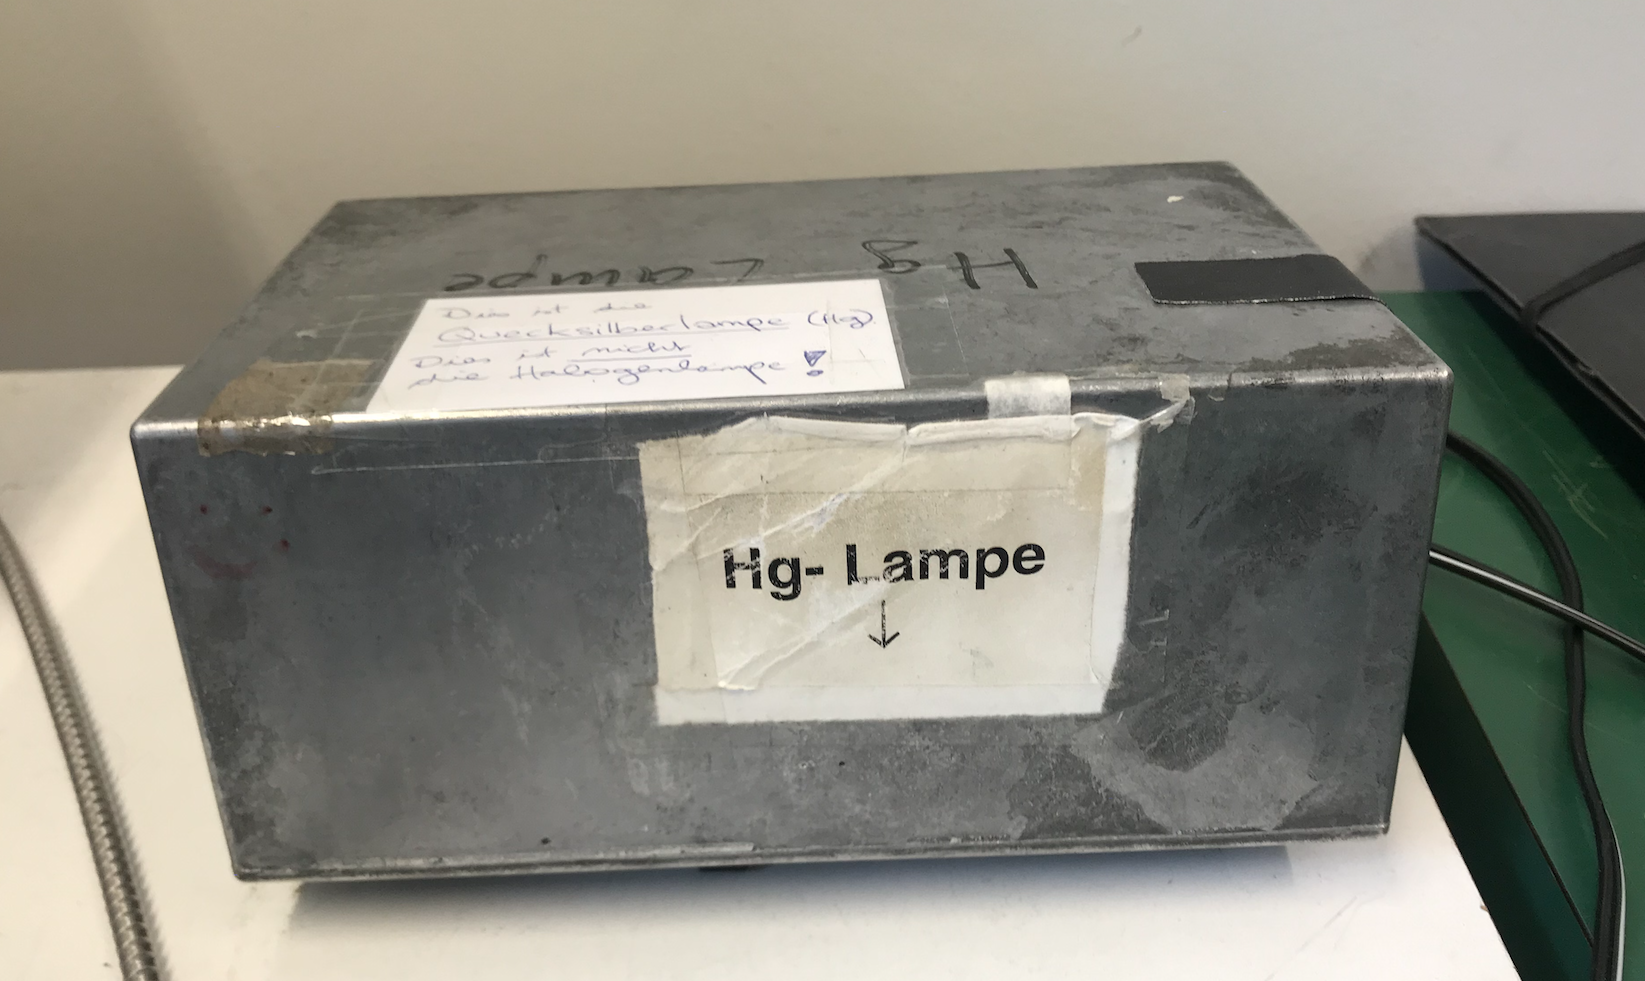
\includegraphics[width=0.5\textwidth]{fig/photo/hg_lampe.png}
    \end{figure}
\end{frame}


\begin{frame}
    \frametitle{Auflösung des Spektrometers} 
    \begin{tabular*}{\linewidth}{@{\extracolsep{\fill}} c c c}
    \toprule
    Maximum & Wellenlänge & FWHM [\si{nm}] \\
    \midrule
    1 & $\sim 313$ & $1.2 \pm 0.1$ \\
    2 & $\sim 365$ & $0.8 \pm 0.1$ \\
    3 & $\sim 404$ & $0.6 \pm 0.1$ \\
    4 & $\sim 436$ & $0.7 \pm 0.1$ \\
    \bottomrule
\end{tabular*}
\end{frame}

\begin{frame}
    \section{Labormessungen}
    \frametitle{Halogenlampen Messung}

    \begin{figure}[h]
        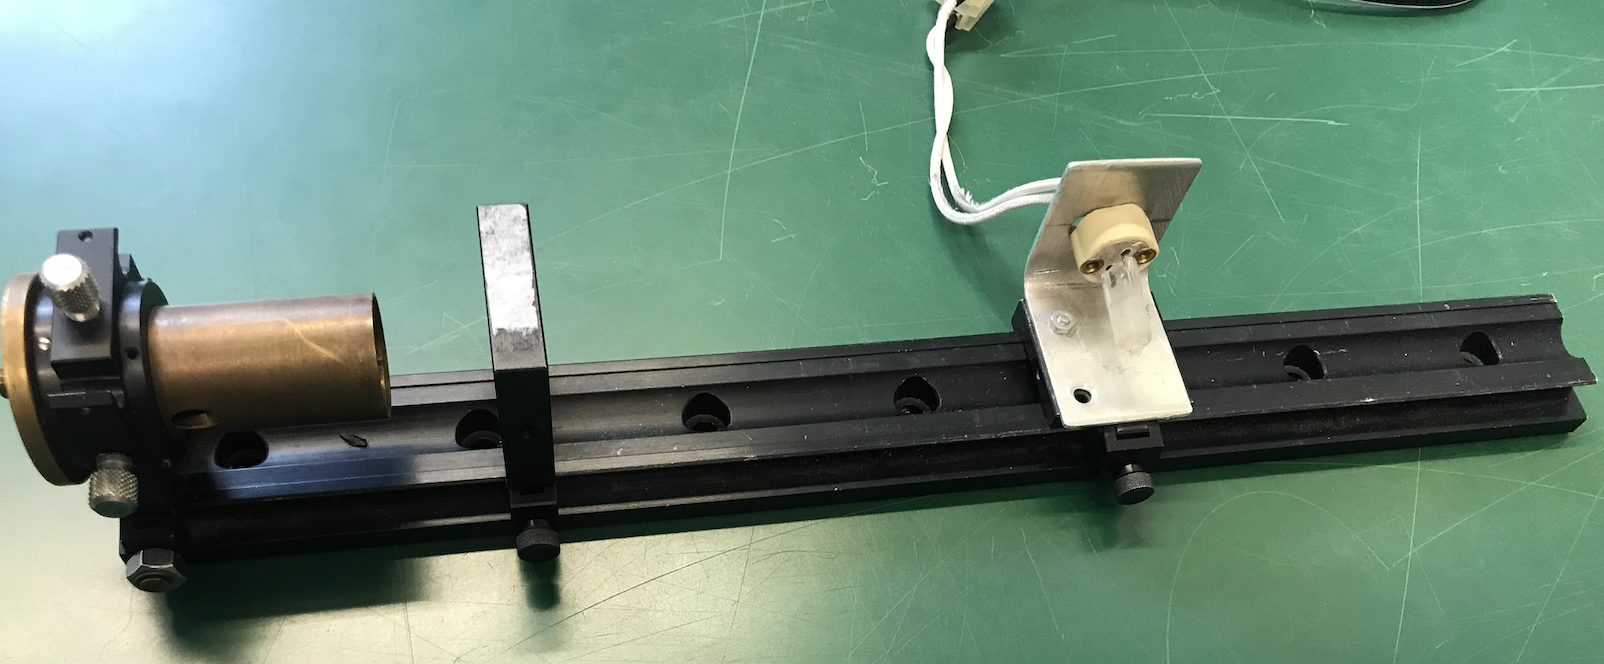
\includegraphics[width=0.5\textwidth]{fig/photo/aufbau_1.png}
    \end{figure}

    \begin{figure}[h]
        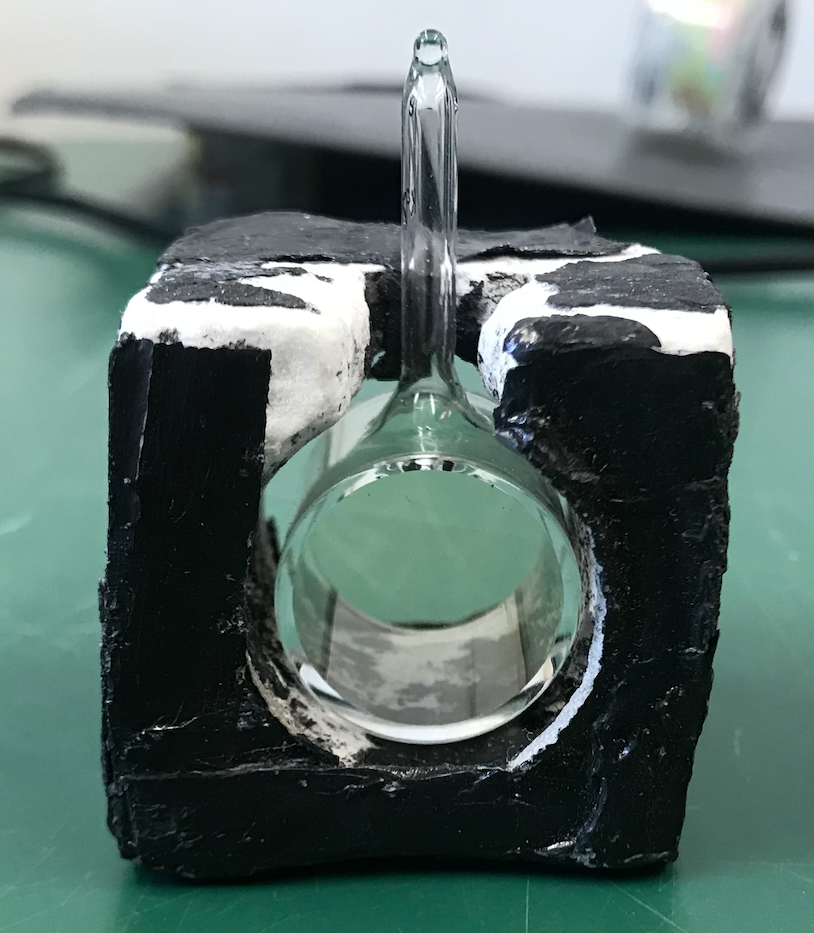
\includegraphics[width=0.5\textwidth]{fig/photo/glas_test.png}
    \end{figure}
\end{frame}

\begin{frame}
    \frametitle{Halogenlampen Messung}
\begin{itemize}
    \item Atmosphärische Einflüsse vernachlässigbar
        \begin{align}
 \to \tau = \sigma_{\ch{NO2}}(\lambda) \cdot     \rho_{\ch{NO2}} \cdot L
        \end{align}
    \item Fitbereich: Suche nach Überlagerung mit \ch{NO2} Referenz
    \item Hier verwendet: $(413.46 - 477.25) \si{nm}$
    \item \begin{align}
            \to \rho_\ch{NO2} = (2.48 \pm 0.12) \cdot 10^20 \si{\frac{\text{Moleküle}}{\ell}}
    \end{align}
\end{itemize}
\end{frame}

\begin{frame}
    \section{Atmosphärische Messungen}
\end{frame}



\end{document}
